\section{Numerical experiments}
\label{sec:experiments}

We first compare the ability of the safe SDG and two residual merits to
recover KKT points, then examine what proximal escape reveals about the
recovered candidates.  Two small problems with complete stationary catalogs
make missed branches identifiable.  The second problem also has analytic
escape radii, allowing the distinction between stationarity and minimality
to be checked without relying on an outer numerical optimizer.

\subsection{Recovering stationary branches}
\label{subsec:experiments-root-recovery}

\subsubsection{Test problems}

The affine rank-one problem has a smooth objective and isolated KKT pairs:
\begin{equation}
  \min_{v_1^\top x=c} f(x)=\frac14\norm{xx^\top-M}_F^2,
  \qquad
  M=V\operatorname{Diag}(d_1,\ldots,d_8)V^\top,
  \qquad c=0.4,
  \label{eq:experiment-affine-rank-one}
\end{equation}
where \(V=[v_1,\ldots,v_8]\) is orthogonal and
\(d_i=4-(i-1)/2\).  In the eigenbasis, stationarity in a free coordinate
requires \((\norm{x}^2-d_j)x_j=0\).  Since the eigenvalues are distinct,
at most one free coordinate is nonzero.  The complete catalog is therefore
\begin{equation}
  \begin{aligned}
    x_0&=cv_1,
    &y_0&=(d_1-c^2)c,\\
    x_j^\pm&=cv_1\pm\sqrt{d_j-c^2}\,v_j,
    &y_j^\pm&=(d_1-d_j)c,\quad j=2,\ldots,8.
  \end{aligned}
  \label{eq:experiment-affine-oracle}
\end{equation}
At \(x_0\), the Hessian restricted to \(\ker A\) has eigenvalues
\(c^2-d_k<0\), \(k\ge2\).  At \(x_j^\pm\), they are
\(2(d_j-c^2)\) and \(d_j-d_k\), \(k\ge2\), \(k\ne j\).
Thus \(x_0\) is a strict constrained local maximum, the twelve points
with \(j\ge3\) are strict saddles, and the two points with \(j=2\)
are minima.  They are global: at a fixed norm of the free component,
the Rayleigh bound selects \(v_2\), and minimization over that norm
gives \(\sqrt{d_2-c^2}\).
For the reported run, \(V\) is obtained by QR factorization of an
\(8\times8\) standard Gaussian matrix from NumPy's
\texttt{SeedSequence([20260709,1401])}, with the signs chosen so that
the diagonal of \(R\) is positive.

The box problem introduces active constraints and nonglobal local minima:
\begin{equation}
  \min_{\substack{x\in[0,1]^7\\x_1=0.37}}
  F(x)=\sum_{i=1}^7 F_i(x_i),
  \qquad F_i(t)=\frac12q_it^2+r_it.
  \label{eq:experiment-box-qp}
\end{equation}
Here \(B=[0,1]^7\), \(f=F+\ind_B\), and
\(\Cset=\{x:x_1=0.37\}\); hence \(A=e_1^\top\) and \(b=0.37\), where
\(e_i\) denotes the \(i\)th standard coordinate vector.
The quadratic coefficients satisfy \(q_2,q_3,q_4<0\), while all other
\(q_i\) are positive.  Coordinates \(2,3,4\) are therefore concave, with
interior maxima \(a_i=-r_i/q_i\) given by
\((a_2,a_3,a_4)=(0.30,0.335,0.37)\).
The remaining free coordinates are strictly convex with interior minima.
Each concave coordinate has three KKT states, \(0,a_i,1\), denoted by
\(L,I,U\), as illustrated in \Cref{fig:box-states}.  This gives
\(3^3=27\) KKT points: \(19\) constrained strict saddles
and eight local minima.  Here a strict saddle has a negative-curvature
direction tangent to its active face, supplied by any interior concave
coordinate.  Among the endpoint combinations, UUU is the unique global
minimum because
\[
  F_i(1)-F_i(0)=q_i(1/2-a_i)<0,\qquad i=2,3,4.
\]
The other seven local minima cannot be rejected by an arbitrarily small
perturbation.  This feature makes the box problem useful for the radius
comparison in \Cref{subsec:experiments-escape}.

\begin{figure}[htbp]
  \centering
  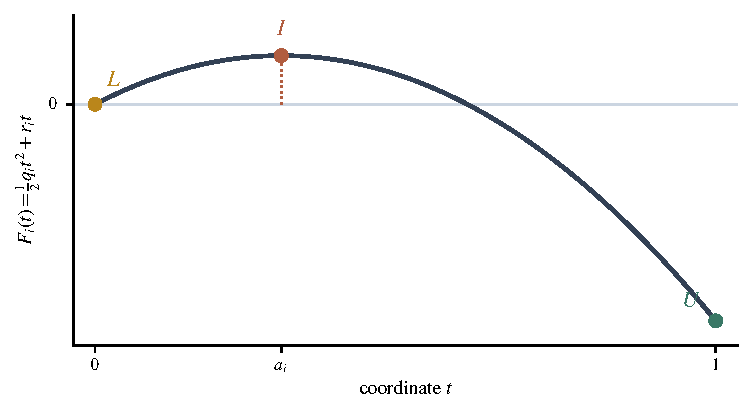
\includegraphics[width=0.69\textwidth]{../experiments/results/figures/box_states.pdf}
  \caption{Three KKT states of a concave box coordinate, illustrated for
  \(i=2\).  The endpoints \(L\) and \(U\) are one-sided local minima;
  \(I\) is an interior maximum.  Since \(a_i<1/2\), \(U\) is globally
  minimizing.  Choosing one state for each of coordinates \(2,3,4\)
  gives the box catalog.}
  \label{fig:box-states}
\end{figure}

Both problems admit inexpensive safe proximal evaluations.  Write
\begin{equation}
  p(x,y)=p_{\beta_x}(x,y)
  =\argmin_u\left\{f(u)+\ip{y}{Au-b}
                    +\frac{\beta_x}{2}\norm{u-x}^2\right\}.
  \label{eq:experiment-lagrangian-prox}
\end{equation}
For the rank-one objective,
\(\nabla^2f(x)=2xx^\top+\norm{x}^2I-M\succeq-4I\);
we use \(\rho=4\) and \(\beta_x=5\).  With
\(z=x-\beta_x^{-1}yv_1\), \(\widehat z=V^\top z\), and
\(\widehat p=V^\top p(x,y)\), its evaluation reduces to
\begin{equation}
  \sum_{i=1}^8
    \left(\frac{\beta_x\widehat z_i}{\beta_x+s-d_i}\right)^2-s=0,
  \qquad
  \widehat p_i=\frac{\beta_x\widehat z_i}{\beta_x+s-d_i}.
  \label{eq:experiment-secular-prox}
\end{equation}
Writing the scalar left-hand side as \(\varphi(s)\), one has
\(\varphi'(s)<-1\) for a nonzero center.  Starting from
\([0,\max\{1,\norm z^2\}]\), the upper endpoint is doubled until
\(\varphi\le0\), then Brent's method is applied with absolute tolerance
\(10^{-13}\) and relative tolerance \(2\cdot10^{-14}\); the zero center
returns zero directly.  For an approximate root \(s\), its point
\(p(s)=V\widehat p(s)\) satisfies
\(\nabla q_{x,y}(p(s))=\varphi(s)p(s)\), so the scalar residual yields
the inner stationarity residual used in \Cref{lem:inexact-safe-prox}.
For the box objective \(f=F+\ind_B\), we use
\(\rho=-\min_i q_i\simeq2.24\) and \(\beta_x=3\), giving
\begin{equation}
  p_{B,i}(x,y)=\Pi_{[0,1]}
  \left(\frac{\beta_xx_i-r_i-y\,\mathbf1_{\{i=1\}}}{\beta_x+q_i}\right).
  \label{eq:box-branch-prox}
\end{equation}
This map enforces the box but dualizes the equality.  The escape test,
in contrast, will enforce both constraints in its proximal evaluation.

\subsubsection{Merit comparison and branch coverage}

We compare the SDG with the squared Lagrangian-proximal and KKT residuals:
\begin{align}
  M_{\rm SDG}(x,y)&=\G_{\beta_x,\beta_y}(x,y),\nonumber\\
  M_{\rm prox}(x,y)&=\frac12\left(
    \beta_x^2\norm{x-p(x,y)}^2+\norm{Ax-b}^2\right),\nonumber\\
  M_{\rm KKT}(x,y)&=\frac12\left(
    \norm{\nabla f(x)+A^\top y}^2+\norm{Ax-b}^2\right).
  \label{eq:experiment-merit-functions}
\end{align}
For the box problem, \(M_{\rm prox}\) uses \(p_B\), while the KKT
stationarity residual is replaced by the natural mapping
\[
  N_B(x,y)=x-\Pi_B\bigl(x-\nabla F(x)-e_1y\bigr).
\]
The self-centered SDG (SC-SDG) uses the smooth finite extension in
\Cref{prop:finite-box-sdg-extension}, minimized over
\(x\in B\), \(y\in\R\).  These are the actual outer bounds:
the primal variables stay in the box, whereas the multiplier is unbounded.
All three merits have the same KKT
zero set; the comparison concerns how readily local minimization reaches
different parts of that set.

Each merit is minimized with L-BFGS-B
\citep{ByrdLuNocedalZhu1995,VirtanenEtAl2020}, using \(\beta_y=1\) and
identical starts within each problem.  The affine comparison uses \(160\)
isotropic primal starts with log-uniform radii in \([0.08,3.2]\) and
Gaussian multipliers of standard deviation \(1.8\).  The box comparison
uses \(256\) scrambled Sobol' points \citep{Owen1998}, generated with
SciPy's linear-matrix scramble and digital shift, in
\([0,1]^7\times[-4,4]\); this multiplier interval applies only to
initialization.  Affine iterates are unbounded in both variables.
The master seed is \(20260709\).  The catalogs are used only to assess endpoints,
not to initialize the searches.  Analytic gradients are supplied for the
smooth merits; the other box merits use piecewise-analytic derivatives,
with clipping derivative zero at a transition.  We use CPython 3.14.0,
NumPy 2.3.5 and SciPy 1.16.3, with \texttt{ftol=1e-15} and
\texttt{gtol=2e-10}.  The iteration limits are \(320\) and \(1000\), and
the line-search limits are \(40\) and \(60\), respectively; the affine
run also sets \texttt{maxfun=320}.

Endpoints are accepted only if independently recomputed, normalized
feasibility, stationarity, and proximal residuals are at most \(10^{-7}\);
the box test also checks the hard-constrained proximal residual.  In the
affine case, these three quantities are
\begin{equation}
  \frac{\norm{Ax-b}}{1+\norm b},\qquad
  \frac{\norm{\nabla f(x)+A^\top y}}{1+\norm{\nabla f(x)}+\norm{A^\top y}},
  \qquad
  \frac{\beta_x\norm{x-p(x,y)}}{1+\beta_x\norm x+\norm{A^\top y}}.
  \label{eq:affine-audit-residuals}
\end{equation}
For the box, the four tests use
\begin{equation}
  \frac{|x_1-0.37|}{1.37},\quad
  \frac{\norm{N_B(x,y)}}{1+\norm{x}},\quad
  \frac{\beta_x\norm{x-p_B(x,y)}}{1+\beta_x\norm x},\quad
  \frac{\beta_x\norm{x-P_{1/\beta_x}^{\Cset}(x)}}{1+\beta_x\norm x}.
  \label{eq:box-audit-residuals}
\end{equation}
The box normalizations depend only on the primal point, so increasing the
multiplier cannot suppress a saturated projection residual.
Acceptance does not depend on the optimizer's success flag.  An accepted
endpoint is assigned to its nearest catalog pair in joint Euclidean
\((x,y)\) distance, with tolerance
\(8\cdot10^{-5}(1+\norm{(x,y)})\) at the affine endpoint and absolute tolerance
\(2\cdot10^{-5}\) for the box problem.  Repeated matches count once in
branch coverage.  Every accepted endpoint in this run also matches its
catalog; there are no accepted unmatched endpoints.

\begin{table}[htbp]
  \centering
  \caption{KKT recovery from common starts.  Accepted endpoints pass the
  independent residual tests; distinct roots count different catalog matches.}
  \label{tab:root-recovery}
  \small
  \setlength{\tabcolsep}{6pt}
  \begin{tabular}{@{}llcc@{}}
    \toprule
    Family & Search objective & Accepted endpoints & Distinct roots\\
    \midrule
    % Generated by python -m sdg_report_experiments; do not edit by hand.
\multirow{3}{*}{affine rank one} & SC--SDG & 159/160 & 15/15 \\
 & Lagrangian prox residual & 160/160 & 15/15 \\
 & KKT residual & 160/160 & 15/15 \\
\midrule
\multirow{3}{*}{box QP} & SC--SDG & 101/256 & 27/27 \\
 & Lagrangian prox residual & 109/256 & 10/27 \\
 & natural KKT residual & 33/256 & 16/27 \\
\bottomrule

  \end{tabular}
\end{table}

In this run, all three merits recover the fifteen affine KKT pairs
(\Cref{tab:root-recovery}).  On the box problem, SC-SDG recovers all
\(27\) branches, compared with \(10\) for the proximal residual and \(16\)
for the natural KKT residual.  All methods find the eight local minima;
their saddle coverage is respectively \(19/19\), \(2/19\), and \(8/19\).
The proximal residual accepts more endpoints than SC-SDG but finds fewer
branches, illustrating why endpoint success alone is not a sufficient
measure of coverage.

The box result favors SC-SDG for this common-start L-BFGS-B comparison.
It also reflects a regularity difference: unlike the other two box
merits, SC-SDG does not require differentiating the clipping map.
The comparison uses one seed and one Sobol scramble, so the observed
coverage reflects both the merit and its interaction with L-BFGS-B.
The endpoint counts are also sensitive to floating-point details: the run in
\Cref{tab:root-recovery} was made on Windows~11 with CPython~3.14, and with
the same pinned NumPy, SciPy and Matplotlib versions on macOS (arm64,
CPython~3.11) one affine SC-SDG start (start~45) ends just inside the
acceptance tolerance, giving \(160/160\) instead of \(159/160\); all
\(768\) box endpoints and every distinct-root count are unchanged.

\subsection{Distinguishing the recovered candidates}
\label{subsec:experiments-escape}

\subsubsection{Exact escape radii on the box problem}

We now assess the exact analytic representatives of the matched box
branches, not the floating-point endpoints themselves.  The radii below
are properties of these catalog points.  Descent from an approximate
endpoint rejects only that endpoint; a small matching distance does not
transfer the conclusion to its analytic branch.  For example, for
\(f(t)=t^2\), the exact minimum \(0\) has infinite escape radius, while
every nonzero nearby point has radius zero.
For \(\lambda=1/3\), the hard-constrained proximal map is
\begin{equation}
  P_\lambda^{\Cset}(z)_1=0.37,\qquad
  P_\lambda^{\Cset}(z)_i
  =\Pi_{[0,1]}\left(\frac{z_i-\lambda r_i}{1+\lambda q_i}\right),
  \quad i=2,\ldots,7.
  \label{eq:box-exact-prox}
\end{equation}
Since \(\lambda\rho\simeq0.747<1\), the denominators are positive and
the proximal point is unique.  For a catalog point \(x\), let
\[
  I(x)=\{i\in\{2,3,4\}:x_i=a_i\},\qquad
  L(x)=\{i\in\{2,3,4\}:x_i=0\}.
\]

\begin{proposition}[Exact escape radii for the box benchmark]
  \label{prop:box-exact-escape}
  The escape radius of every KKT point of
  \cref{eq:experiment-box-qp} is
  \begin{equation}
    r_{\lambda}^{\rm esc}(x)
    =
    \begin{cases}
      0,
        & I(x)\ne\varnothing,\\[1mm]
      \displaystyle\min_{i\in L(x)}a_i(2+\lambda q_i),
        & I(x)=\varnothing,\ L(x)\ne\varnothing,\\[2mm]
      +\infty,
        & I(x)=L(x)=\varnothing .
    \end{cases}
    \label{eq:box-exact-radius}
  \end{equation}
\end{proposition}

\begin{proof}
  An arbitrarily small perturbation of an interior concave coordinate is
  mapped away from its scalar maximum and decreases \(F\), proving the first
  case.  At a lower-bound state, the scalar quadratic first reaches an equally
  good point when the proximal output reaches \(2a_i\).  Solving
  \(P_\lambda^{\Cset}(x+\tau_i e_i)_i=2a_i\) gives
  \(\tau_i=a_i(2+\lambda q_i)\).  Before this threshold,
  \(0\le p_i\le2a_i\) and
  \[
    F_i(p_i)-F_i(0)
    =q_i p_i\left(\frac{p_i}{2}-a_i\right)\ge0
  \]
  because \(q_i<0\).  Upper-state concave coordinates and the convex
  coordinates are already at their scalar global minima.  Thus separability
  rules out a cooperative decrease below the smallest threshold, whereas a
  perturbation along a minimizing coordinate produces strict decrease above
  it.  If all concave coordinates are upper-state, every scalar term is
  globally minimized, giving the third case.
\end{proof}

Thus the \(19\) strict saddles have zero escape radius, the seven
nonglobal local minima have positive finite radii, and the global minimum
has infinite radius.  The three possible finite thresholds are approximately
\(0.400\), \(0.433\), and \(0.464\).

\Cref{fig:box-exact-escape} displays one representative of each class.
In IUU and LUU, only coordinate \(2\) can lower the objective, so the
full-ball decrease is obtained from its scalar proximal formula.
For IUU, every positive radius produces a decrease.  For LUU, the decrease
remains zero up to \(a_2(2+\lambda q_2)\), then becomes positive.
The UUU profile stays zero at every radius.

\begin{figure}[htbp]
  \centering
  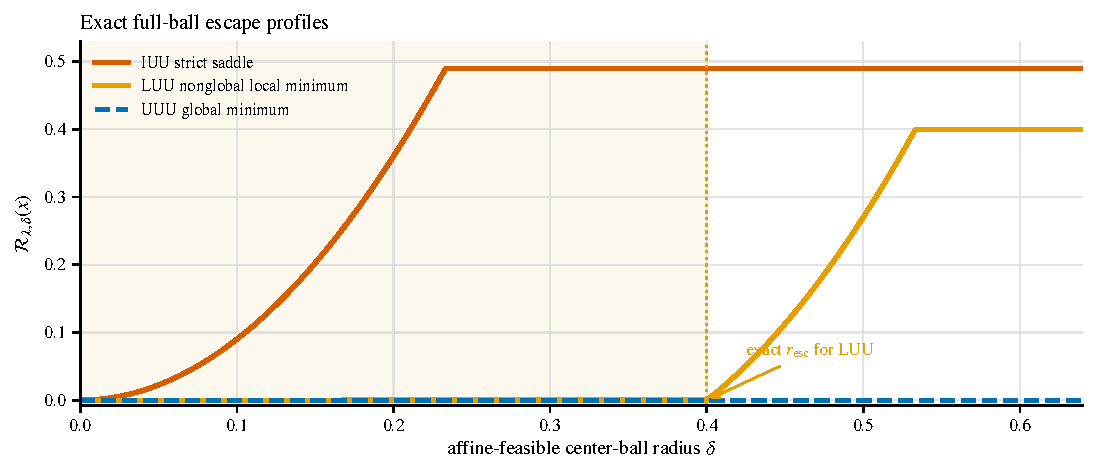
\includegraphics[width=0.88\textwidth]{../experiments/results/figures/box_qp_proximal_escape.pdf}
  \caption{Exact polished-decrease profiles for IUU, LUU, and UUU.
  Their escape radii are zero, approximately \(0.400\), and infinite,
  respectively; \(L,I,U\) denote the lower, interior, and upper states.}
  \label{fig:box-exact-escape}
\end{figure}

The analytic escape test therefore rejects all \(26\) nonglobal catalog
points, verifying the radius classification in
\Cref{thm:radius-classification} through separable scalar calculations.

\subsubsection{A stationary point with vanishing Hessian}

The box saddles already have negative-curvature directions.
To examine a case where a Hessian test is inconclusive, consider on
\(\R^{12}\)
\begin{equation}
  q_3(x)=1+\bigl(\norm{x}^2-1\bigr)^3,
  \qquad \bar x_3=e_1,
  \qquad
  q_{\min}(x)=\norm{x}^4,
  \qquad x_{\min}^\star=0.
  \label{eq:hessian-flat-benchmarks}
\end{equation}
Both base points have zero gradient and zero Hessian.  Nevertheless,
\begin{equation}
  q_3(e_1)-q_3((1-\delta)e_1)
  =(2\delta-\delta^2)^3>0
  \qquad (0<\delta<2),
  \label{eq:hessian-flat-direct-drop}
\end{equation}
whereas \(q_{\min}(x)\ge0=q_{\min}(0)\) for every \(x\).
\Cref{thm:radius-classification}
therefore gives escape radius zero for
\(\bar x_3\) and infinite radius for the flat minimum, although their
first- and second-order data agree.

The radial and tangential Hessian eigenvalues of \(q_3\), with
\(s=\norm{x}^2\), are \(6(s-1)(5s-1)\) and \(6(s-1)^2\).
Their lower bound is \(-24/5\), so we take \(\lambda=1/8\), giving
\(\lambda\rho=0.6\).  We evaluate ten logarithmically spaced radii
between \(10^{-4}\) and \(10^{-1}\), with centers
\(z_j=(1-\delta_j)e_1\).
The relevant proximal model is radial.  More precisely, each center \(z_j\)
and the objective are invariant under
every orthogonal map fixing \(e_1\); uniqueness in the safe regime forces the
proximal point to lie in \(\operatorname{span}\{e_1\}\).  Its scalar coordinate
\(t\) is consequently the unique bracketed root of
\begin{equation}
  6t(t^2-1)^2+8(t-1+\delta)=0.
  \label{eq:hessian-flat-prox-root}
\end{equation}
The derivative of its left-hand side is at least
\(8-24/5=16/5\).  Its signs at \(0\) and \(1-\delta\) are opposite,
so \(0<t_\delta<1-\delta\) for the radii considered.  We use this
bracket in Brent's method, with absolute and relative tolerances
\(10^{-14}\) and \(2\cdot10^{-14}\).  To avoid subtracting objective
values close to one, the plotted decreases are evaluated as
\begin{equation}
  \begin{aligned}
    \Delta_D&=(2\delta-\delta^2)^3,\qquad
    \Delta_P=((1-t_\delta)(1+t_\delta))^3,\\
    \Delta_E&=\Delta_P-4(t_\delta-1+\delta)^2.
  \end{aligned}
  \label{eq:radial-stable-decreases}
\end{equation}
The control \(q_{\min}\) rules out positive decrease analytically for every
\(\lambda>0\), without an inner solve.

The direct, envelope, and polished decreases in
\Cref{fig:experiment-high-order-escape} follow the prescribed radial
direction.  Their positive sign follows from
\cref{eq:hessian-flat-direct-drop} and proximal optimality, independently
of the plotted floating-point values.  Values below
\(100\epsilon_{\rm mach}(1+|q_3(e_1)|)\) are omitted as a reporting convention,
not as an error certificate.

\begin{figure}[htbp]
  \centering
  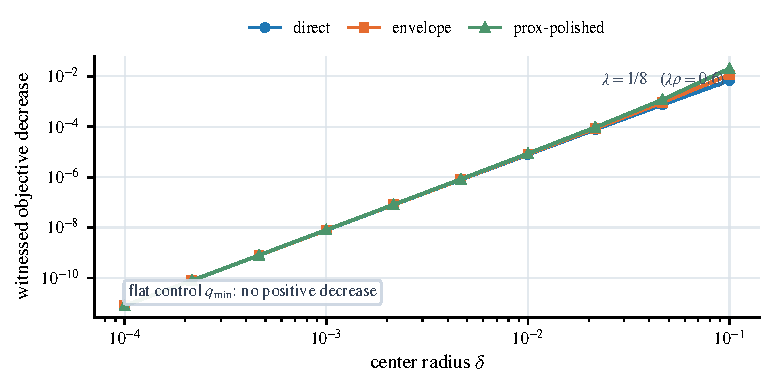
\includegraphics[width=0.72\textwidth]{../experiments/results/figures/experiment_high_order_escape.pdf}
  \caption{Direct, envelope, and polished decreases along
  \(z=(1-\delta)e_1\), with \(\lambda=1/8\).
  The base point has zero gradient and Hessian.  Curves are pathwise
  witnesses, not optimized full-ball values.}
  \label{fig:experiment-high-order-escape}
\end{figure}

Along the analytically supplied direction, proximal escape detects
nonminimality despite a vanishing Hessian.
